 % -*- root: ../main.tex -*-
\documentclass[../main.tex]{subfiles}
\begin{document}

\begin{chapter}{Comparaison des profils d'expressions entre l'épiderme caudal et les bourgeons de membres postérieurs}

\begin{section}{Comparaison globale des programmes transcriptionnels régulés par les hormones thyroïdiennes et les glucocorticoïdes}

Dans le cadre de la caractérisation des programmes transcriptionnel spécifiques des \glspl{hlb} et du \gls{tf}, j'ai partitionné les gènes différentiellement exprimé par rapport à la condition "contrôle" dans au moins une condition quelque soit le tissu selon leur profils d'expression.
Cela représente un total de 5392 gènes.
Le résultat de cette classification sous forme de ``heatmap'' est présenté \autoref{fig:comparison-tfc-hlc-de-genes}.
Sur cette figure, il apparaît que la réponse aux deux signaux hormonaux étudiés est en grande partie spécifique de chaque tissus.
En effet, le nombre de gènes régulés dans le \gls{tf} et les \glspl{hlb} est très différent (1363 et 4741 respectivement).
L'intersection de ces deux jeux de donnés révèle 795 gènes en commun.
\par
En terme de proportions, 54,8 \% des gènes sont différentiellement exprimés dans le \gls{tf} alors qu'il ne représente que 4,3 \% dans les \glspl{hlb}.
Pour les gènes ``antagonistes'' alors que leur nombre est similaire dans les deux tissus étudiés (une centaine), il représente 2,4 \% dans les \glspl{hlb} et 9,5 \% dans le \gls{tf}.
Il ressort que 81 gènes ont un profil "antagoniste" ou ``potentié'' dans les deux tissus ce qui correspond à 9 \% de ces gènes dans le \gls{tf} (6 \% du nombre de gènes différentiellement exprimés tout profils confondus) et 25 \% dans les \glspl{hlb} (1,7 \% du nombre de gènes différentiellement exprimés tous profils confondus).
Majoritairement ces gènes sont dans la catégorie des gènes ``potentié'' (8 ``antagonsites'' pour 61 ``potentié'').
Le comportement de certains gènes est particulier puisqu'ils sont ``potentiés'' dans un tissu et ``antagonisés'' dans l'autre (12 gènes) et inversement.
Ceci est à mettre en perspective par rapport au nombre de gènes ne présentant qu'une réponse à la \gls{t3} (358 dans le \gls{tf}, 4394 dans les \glspl{hlb}).
\par
Les résultats présentés dans les deux chapitres précédents montrent que dans les pattes, la majeure partie de l'effet des hormones est tourné vers le métabolisme de lipides et des stéroïdes, le métabolisme des \gls{rna} et le système immunitaire.
Dans ce tissu, les gènes présentant un profil d'expression dénotant une interaction entre les voies de signalisation \gls{ht} et \gls{gc} sont particulièrement enrichis en modulateurs de la réponse immunitaire innée.
De même, dans le \gls{tf}, la majorité de l'interaction entre les \glspl{ht} et les \glspl{gc} affecte la régulation de la prolifération cellulaire et de l'activation du système immunitaire.
Il est intéressant de noter que dans les deux tissus, la majorité de l'enrichissement de termes associés au système immunitaire provient d'une même sous catégorie de profils d'expression, à savoir la potentiation de l'effet répresseur des \glspl{ht} et des \glspl{gc} dans le cadre d'un co-traitement.
\par
Seuls deux gènes sont potentiés dans les \glspl{hlb} et antagonisés dans le \gls{tf} :
EMILIN2 et FGFBP1, deux facteurs extra-cellulaires, le premier étant un composant élastique de la matrice extra-cellulaire et le second se liant aux facteurs de croissance FGF pour potentier leur action.
De même, 9 gènes sont ``potentiés'' dans le \gls{tf} et ``antagonisés'' dans les \glspl{hlb}.
Ils couvrent des fonctions biologiques allant du contrôle du cycle cellulaire (MOB2, MCM2) au métabolisme des lipides (PNPLA2) en passant par le système immun (NMI) ou encore le remodelage de la matrice extra-cellulaire (ADAMTSL5).

% BOTTOM caption
% ------------------------
\begin{figure}[b]
\centering
\vspace{1\baselineskip}
\includegraphics[width=\textwidth]
% ------------------------
%
% SIDE caption
% ------------------------
%\begin{SCfigure}[\sidecaptionrelwidth][!htbp]
%\centering
%\vspace{1\baselineskip}
%\includegraphics[width=0.5\textwidth]
% ------------------------
%
% Main information
% ===========================================================
{Figures/comparison-tfc-hlc-de-genes/comparison-tfc-hlc-de-genes.pdf}
\caption[Heatmap des profils d'expression des gènes différentiellement exprimés dans au moins une condition]
{
Heatmap des profils d'expression des gènes différentiellement exprimés dans au moins une condition (pattes et queue confondues, 5392 gènes).
Chaque ligne correspond à un gène.
Chaque colonne correspond à un traitement dans les deux tissus considérés (\gls{tf}: ".TFC" \gls{hlb}: ".HLC").
L'intensité des couleurs rouge et bleues est proportionnelle au facteur d'induction de l'expression en $\log_2$ d'un gène donné dans un tissus donné et dans un traitement donné par rapport à la condition "contrôle" (CTRL.TFC et CTRL.HLC).
Les facteurs d'induction ont été plafonnés à 4 afin que le contraste ne soit pas capturer par les gènes les plus fortement exprimés.
La similarité des profils d'expression des gènes est exprimées en fonction de leur distance euclidienne.
Cette mesure permet leur regroupement au sein de la figure.
Le niveau d'expression des gènes qui ne sont pas exprimés dans un tissu est fixé à zéro et apparaissent en gris à travers les quatre traitements.
}
\label{fig:comparison-tfc-hlc-de-genes}
% ===========================================================
%
% BOTTOM caption
% ------------------------
\end{figure}
% ------------------------
%
% SIDE caption
% ------------------------
%\end{SCfigure}
% ------------------------

\end{section}


\begin{section}{Vieillissement}

Comme spécifié précédement, une perturbation du signal thyroïdien durant la période périnatale ou la métamorphose peut avoir des conséquences délétères sur le long terme.
J'ai donc sélectionné un ensemble de gènes impliqués dans un vieillissement prématuré des structures et fonctions biologiques à partir de la base de données HAGR \citep{DeMagalhaes2005}.
Les profils d'expression de 222 orthologues (sur 289) sont présentés \autoref{subfig:comparison-tfc-hlc-aging-all}.
Parmi les 222 gènes, 10 ont une expression spécifique du \glspl{tf} ou des \glspl{hlb}.

% BOTTOM caption
% ------------------------
\begin{figure}[!htbp]
\centering
\vspace{1\baselineskip}
% ------------------------
%
% SIDE caption
% ------------------------
%\begin{SCfigure}[\sidecaptionrelwidth][!htbp]
%\centering
%\vspace{1\baselineskip}
%\includegraphics[width=0.5\textwidth]
% ------------------------
%
% Main information
% ===========================================================
\begin{subfigure}{0.49\textwidth}
	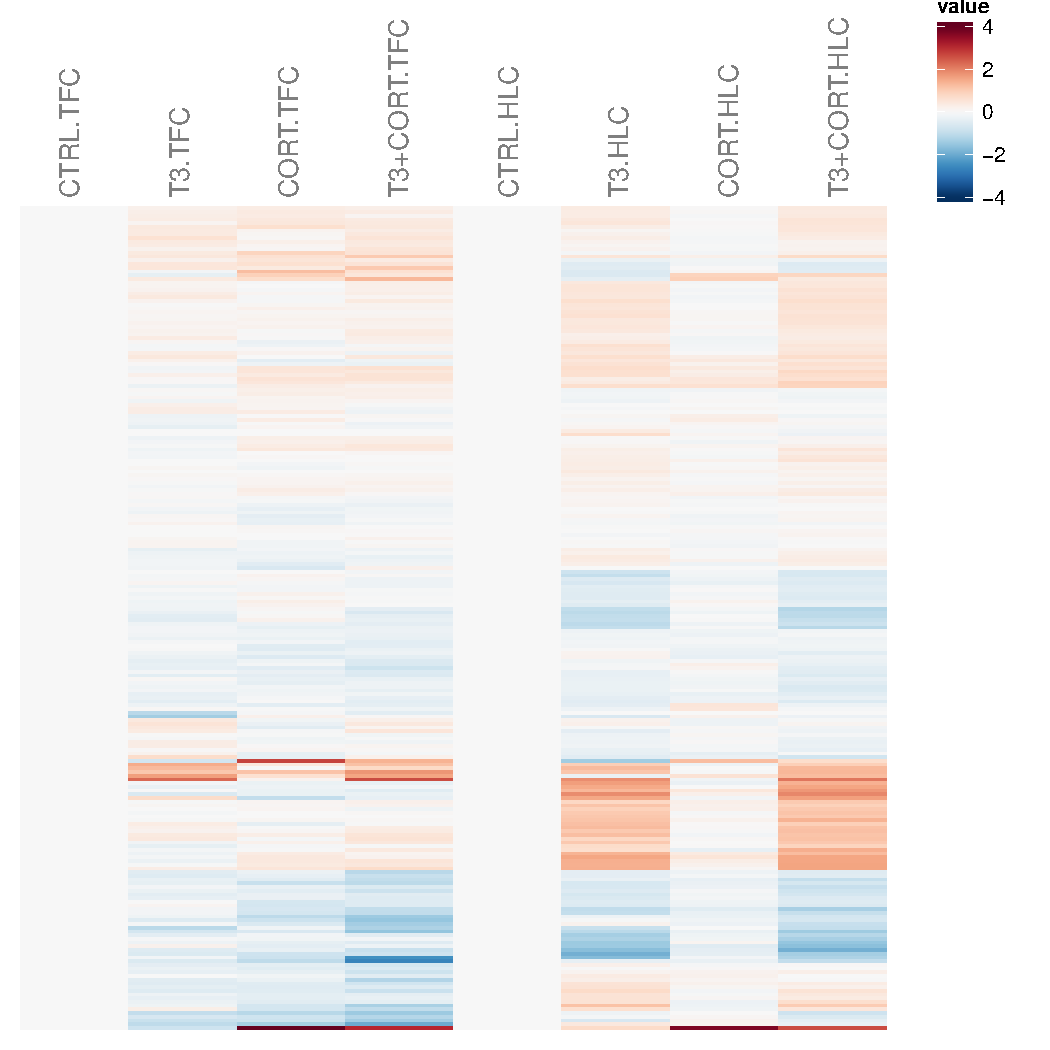
\includegraphics[width=\textwidth]
	{Figures/comparison-tfc-hlc-aging/comparison-tfc-hlc-aging-all.pdf}
	\caption{}
	\label{subfig:comparison-tfc-hlc-aging-all}
\end{subfigure}
\begin{subfigure}{0.49\textwidth}
	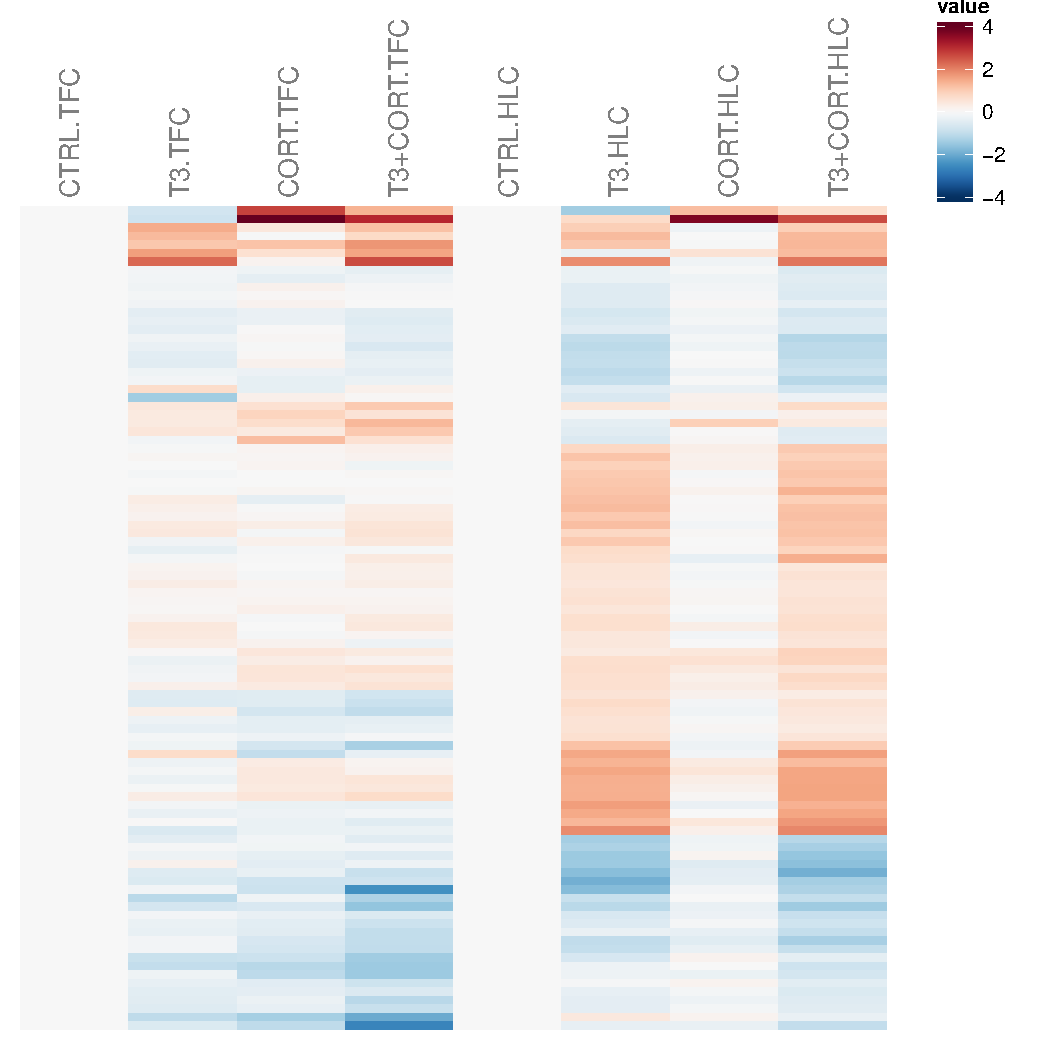
\includegraphics[width=\textwidth]
	{Figures/comparison-tfc-hlc-aging/comparison-tfc-hlc-aging-de.pdf}
	\caption{}
	\label{subfig:comparison-tfc-hlc-aging-de}
\end{subfigure}
\caption[Profils d'expression des gènes impliqués dans le vieillissement]
{
Comparaison des profils d'expression, dans l'épiderme caudal et les bourgeons de membres postérieurs, des gènes impliqués dans le vieillissement.
\ref{subfig:comparison-tfc-hlc-aging-all} Tous les gènes.
\ref{subfig:comparison-tfc-hlc-aging-de} Sélection des gènes différentiellement exprimés dans au moins une condition (présentés \autoref{fig:comparison-tfc-hlc-de-genes}).
}
\label{fig:comparison-tfc-hlc-aging}
% ===========================================================
%
% BOTTOM caption
% ------------------------
\end{figure}
% ------------------------
%
% SIDE caption
% ------------------------
%\end{SCfigure}
% ------------------------

Après avoir filtré ce set de gène pour ne conserver que ceux qui sont différentiellement exprimés dans au moins une condition (97 gènes), il apparait une dichotomie entre les deux tissus:
Alors que dans les \gls{hlb} 87 gènes sont affectés par au moins un des traitements hormonaux, seuls 25 le sont dans le \gls{tf} (\autoref{subfig:comparison-tfc-hlc-aging-de}).
Dans le \gls{tf}, la 10 gènes sont spécifiques de ce tissu alors que 72 sont spécifiques des \glspl{hlb}. 
De plus, tout tissu confondu, 72, 6 et 86 gènes sont régulés par la \gls{t3}, la \gls{cort} et le co-traitement avec les deux hormones.
\par
Parmi les gènes dont l'expression présente un profil d'``antagonisme'' ou de ``potentiation'' \glspl{ht} et les \glspl{gc}, on trouve entre autres les orthologues de \gls{stat5}B ($log_2(FC)=-0,11$ ; $1,23$ ; $0,66$ dans les traitements \gls{t3}, \gls{cort} et \gls{t3}+\gls{cort} respectivement), FOXO3 ($log_2(FC)=0,43$ ; $0,61$ ; $1,04$), IGF1R ($log_2(FC)=1,28$ ; $-0,03$ ; $0,78$) ; GHR ($log_2(FC)=-1,40$ ; $0,20$ ; $0,05$), RAD51 ($log_2(FC)=-0,98$ ; $-1,12$ ; $-1,46$) dans le \gls{tf}, \gls{cebpa} ($log_2(FC)=-0,25$, $0,57$, $1,24$), LEPR ($log_2(FC)=-1,40$, $1,23$, $0,70$) dans les \glspl{hlb}.
\par
\gls{socs2} est induit par la \gls{t3} dans les \glspl{hlb} ($log_2(FC)=1,16$, $-0,20$, $1,01$ dans les traitements \gls{t3}, \gls{cort} et \gls{t3}+\gls{cort} respectivement) et réprimé de façon ``potentialisée'' par les deux hormones dans le \gls{tf} ($log_2(FC)=-0,17$, $-0,72$, $-1,30$).
Dans les deux tissus, l'induction de PCK1 \gls{cort}-dépendante (($log_2(FC)=3,74$ et $5,00$ dans les \glspl{hlb} et le \gls{tf} respectivement) est antagonisée par la \gls{t3} (($log_2(FC)=2,67$ et $3,10$ respectivement).

\end{section}


\begin{section}{Les modificateurs post-traductionnels des histones}\label{sec:res-histones}

Outre une action sur la mise en place des structures anatomiques et morphologiques, une perturbation de la signalisation thyroïdienne pourrait affecter la présence de modificateurs de la chromatine et influer sur la spécificité spatiale et temporelle de déposition des marques.
J'ai donc séléctionné sur la base de leur annotation \gls{go}, les gènes impliqués dans la (dés)acétylation et la (dé)méthylation des histones.
La liste initiale comprend 241 gènes humains pour lesquels un orthologue chez le Xénope a pu être identifié.
Dans le \gls{tf} et les \glspl{hlb}, 203 et 205 gènes respectivement sont exprimés (passent l'étape de ``filtre indépendant'', voir \autoref{subsec:diff-expr-call}), pour un total de 209 gènes.
La \autoref{subfig:comparison-tfc-hlc-histones-all} présente les profils d'expression de l'ensemble de ces gènes.
Exceptés quelques sous ensembles de gènes et indépendamment de leur significativité d'expression différentielle, les profils d'expression entre le \gls{tf} et les \gls{hlb} restent similaires.

% BOTTOM caption
% ------------------------
\begin{figure}[!htbp]
\centering
\vspace{1\baselineskip}
% ------------------------
%
% SIDE caption
% ------------------------
%\begin{SCfigure}[\sidecaptionrelwidth][!htbp]
%\centering
%\vspace{1\baselineskip}
%\includegraphics[width=0.5\textwidth]
% ------------------------
%
% Main information
% ===========================================================
\begin{subfigure}{0.495\textwidth}
	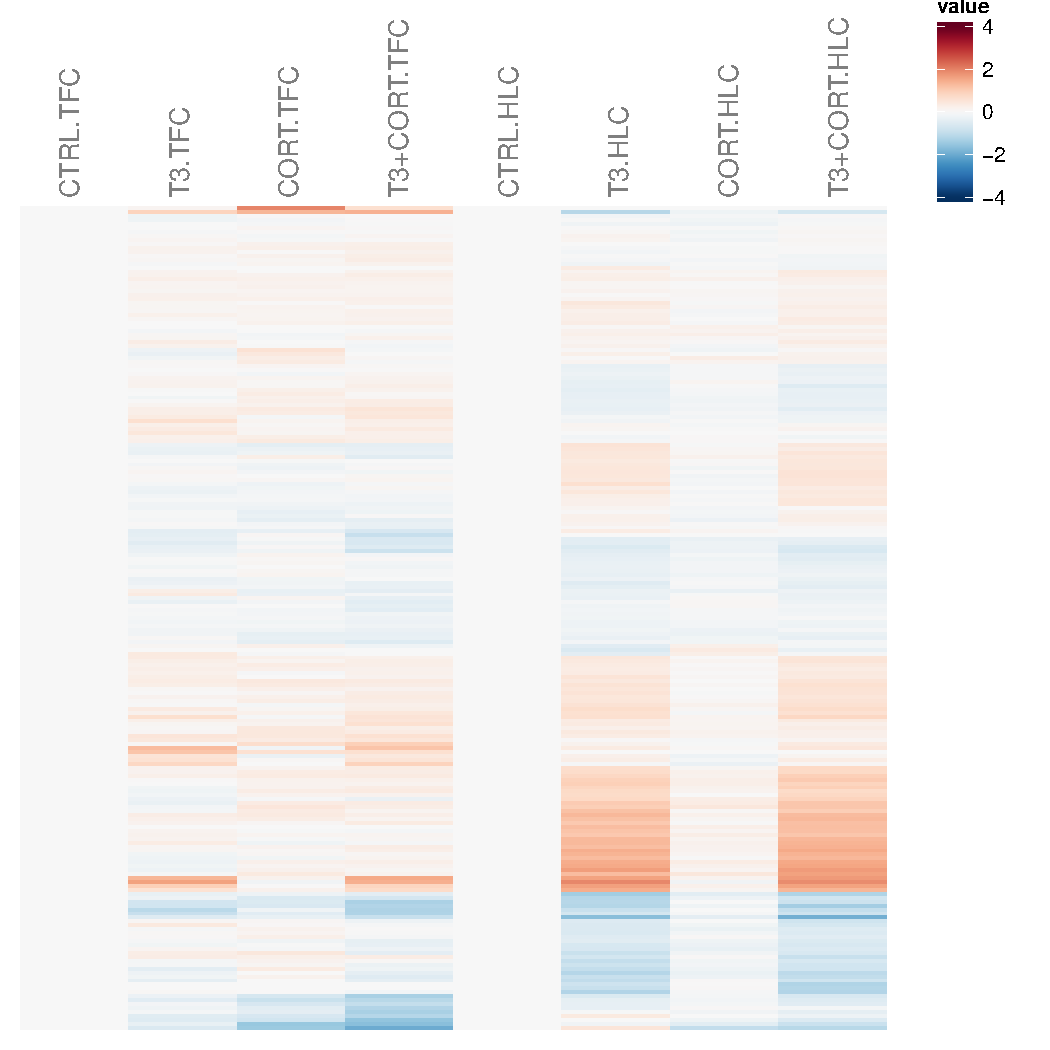
\includegraphics[width=\textwidth]
	{Figures/comparison-tfc-hlc-histones/comparison-tfc-hlc-histones-all.pdf}
	\caption{}
	\label{subfig:comparison-tfc-hlc-histones-all}
\end{subfigure}
\begin{subfigure}{0.495\textwidth}
	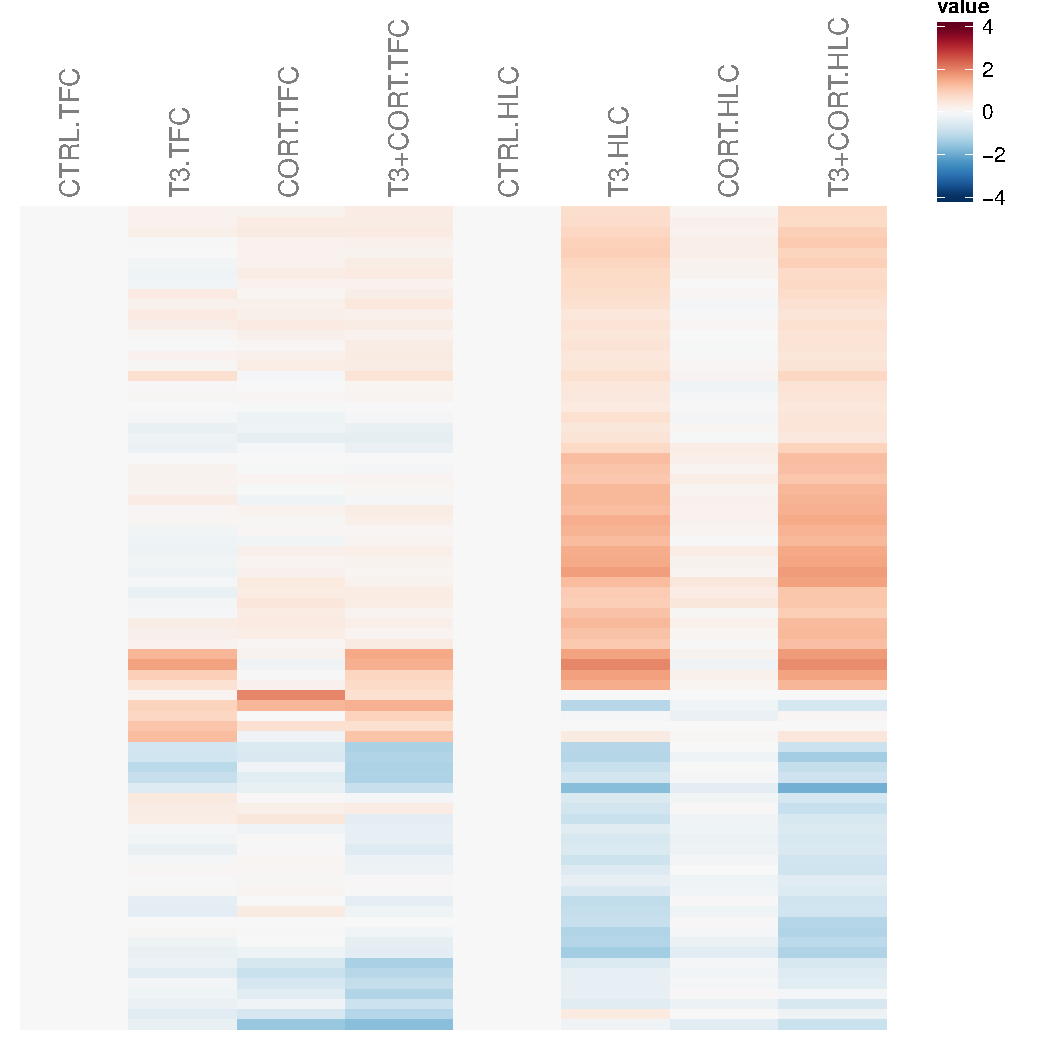
\includegraphics[width=\textwidth]
	{Figures/comparison-tfc-hlc-histones/comparison-tfc-hlc-histones-de.pdf}
	\caption{}
	\label{subfig:comparison-tfc-hlc-histones-de}
\end{subfigure}
\caption[Profils d'expression des gènes impliqués dans la modification d'histones]
{
Comparaison des profils d'expression, dans l'épiderme caudal et les bourgeons de membres postérieurs, des gènes impliqués dans les modifications post-traductionnelles d'histones.
\ref{subfig:comparison-tfc-hlc-histones-all}: Tous les gènes.
\ref{subfig:comparison-tfc-hlc-histones-de}: Sélection des gènes différentiellement exprimés dans au moins une condition.
}
\label{fig:comparison-tfc-hlc-histones}
% ===========================================================
%
% BOTTOM caption
% ------------------------
\end{figure}
% ------------------------
%
% SIDE caption
% ------------------------
%\end{SCfigure}
% ------------------------

La \autoref{subfig:comparison-tfc-hlc-histones-de} présente uniquement les gènes différentiellement exprimés dans au moins une condition.
Cela représente 17 gènes dans le \gls{tf} et 73 gènes dans les \gls{hlb}, pour un total de 80 gènes.
Il ressort que la majorité des gènes ne sont différentiellement exprimés que dans les \gls{hlb}.
De façon intéressante, là encore le chevauchement entre les deux sous ensembles de gènes est restreint et souligne ici une spécificité tissulaire de la réponse.
Nous remarquons par exemple que \gls{jhdm1d} est, sous l'effet de la \gls{t3}, réprimé dans les \glspl{hlb} ($log_2(FC)=-1,14$ ; $-0,17$ ; $-0,70$) mais induit dans le \gls{tf} sous l'effet de la \gls{t3} et de la \gls{cort} ($log_2(FC)=0,89$ ; $1,35$ ; $1,40$).
NSD1 n'est induit par la \gls{t3} dans les \glspl{hlb} ($log_2(FC)=1,30$ ; $0,17$ ; $1,37$), de même que TRRAP ($log_2(FC)=1,14$ ; $0,1$ ; $1,19$).
\par
Les gènes catégorisés comme cible d'une interaction entre \glspl{ht} et \glspl{gc} et impliqués dans la modification des histones incluent 6 gènes :
CDK2 (potentié : $log_2(FC)=-0,48$ ; $-0,66$ ; $-1,15$), GFI1B (induction \gls{cort}-dépendante antagonisée par la \gls{t3} : $log_2(FC)=0,09$ ; $1,97$ ; $0,63$), PRKCB ($log_2(FC)=-0,16$ ; $-0,42$ ; $-1,20$), PHF15 (réprimé de façon ``potentiée'' $log_2(FC)=-0,76$ ; $-0,57$ ; $-1,28$), MECP2 ($log_2(FC)=-0,92$ ; $-0,44$ ; $-1,22$),  et SATB1 (réprimé de façon ``potentiée'' : $log_2(FC)=-0,22$ ; $-0,69$ ; $-1,30$).
Dans les \gls{hlb}, aucun gène impliqué dans un effet croisé de la \gls{t3} et de la \gls{cort} ne semble impliqué dans la modification des histones.
Enfin, il est important de mentionner que certains gènes dans cette catégorie (et la suivante) paraissent au premier abord mal catégorisés.
La raison est que les listes de gènes ont été obtenues programmatiquement en utilisant la \gls{go}.
Ainsi, MECP2, connu pour être essentiel dans la lecture de l'\gls{dna} méthylé, n'est pas à strictement parlé impliqué dans les processus de méthylation de l'\gls{dna}.
Il a été en revanche associé à la favorisation du dépôt de certains modifications d'histones en fonction de l'état de méthylation d'un locus \citep{Fuks2003}.

\end{section}


\begin{section}{La méthylation de l'ADN}

La modification de l'épigénome peut aussi se traduire par la méthylation de l'\gls{dna} au niveau d'îlots CpG, en général associés à la répression de la transcription.
De même que ce qui a été effectué dans la section précédente, j'ai séléctionné 43 gènes impliqués dans les processus de méthylation de l'\gls{dna}, dont 33 sont exprimés dans les tissus étudiés, avec 1 gène spécifiquement exprimé dans les \glspl{hlb}.
Leurs profils d'expression sont présentés \autoref{subfig:comparison-tfc-hlc-medna-all}.

% BOTTOM caption
% ------------------------
\begin{figure}[!htbp]
\centering
\vspace{1\baselineskip}
% ------------------------
%
% SIDE caption
% ------------------------
%\begin{SCfigure}[\sidecaptionrelwidth][!htbp]
%\centering
%\vspace{1\baselineskip}
%\includegraphics[width=0.5\textwidth]
% ------------------------
%
% Main information
% ===========================================================
\begin{subfigure}{0.45\textwidth}
	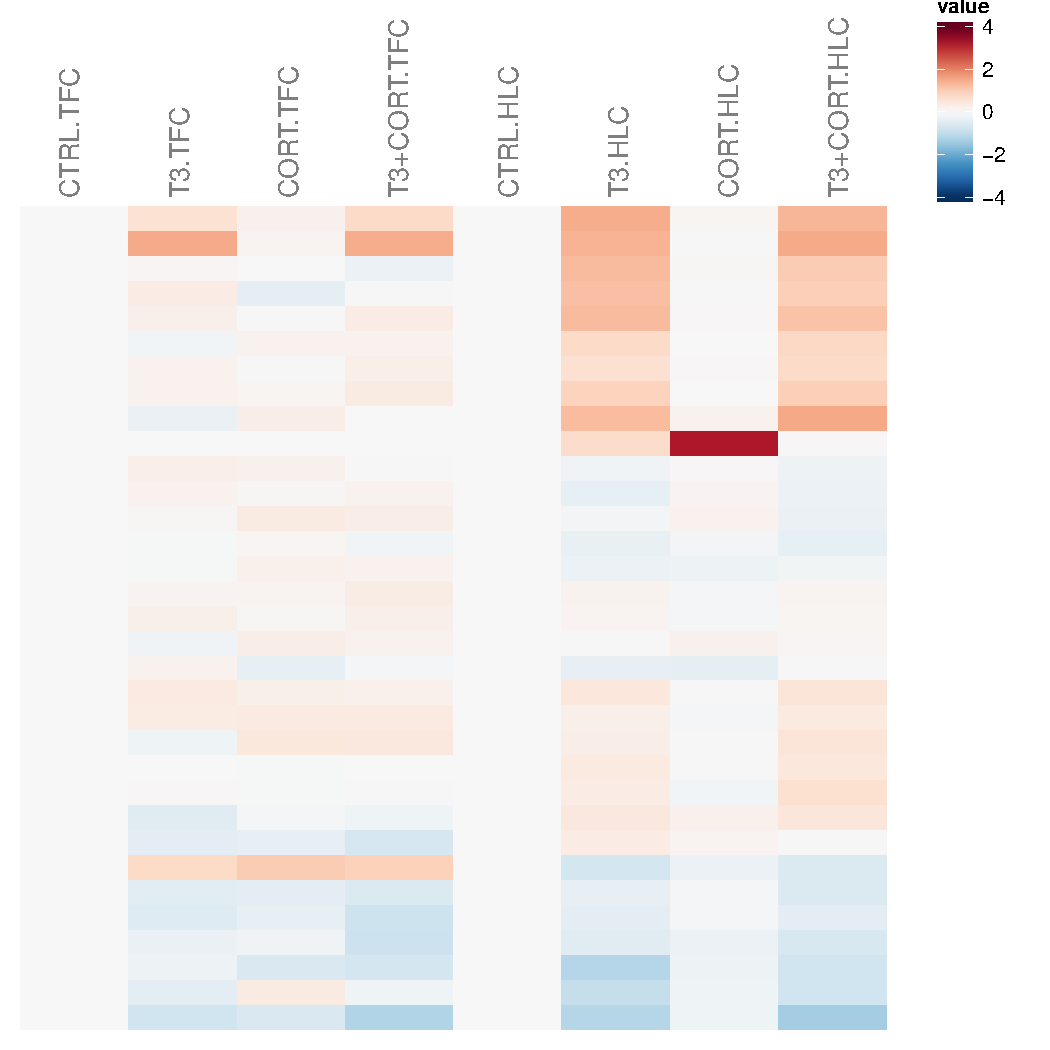
\includegraphics[width=\textwidth]
	{Figures/comparison-tfc-hlc-medna/comparison-tfc-hlc-medna-all.pdf}
	\caption{}
	\label{subfig:comparison-tfc-hlc-medna-all}
\end{subfigure}
~
\begin{subfigure}{0.45\textwidth}
	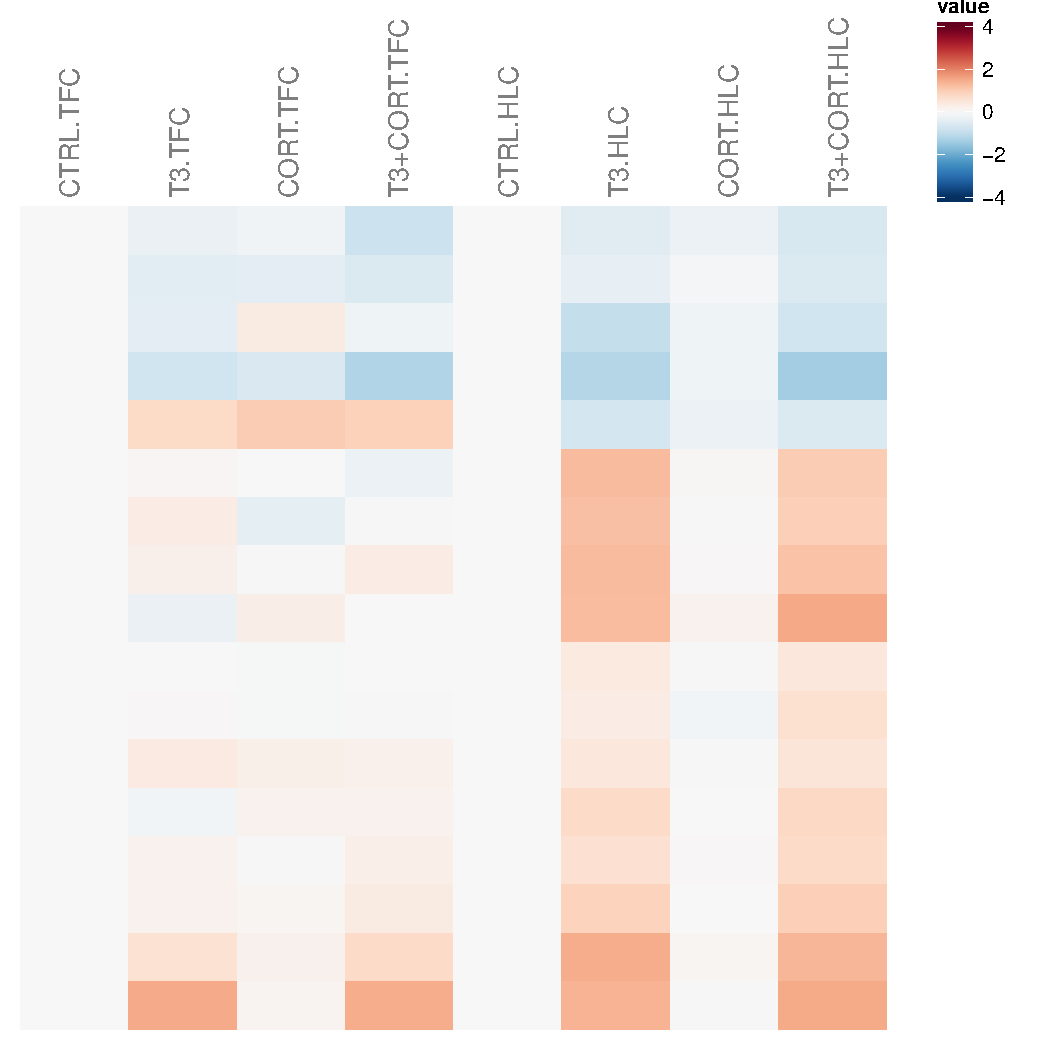
\includegraphics[width=\textwidth]
	{Figures/comparison-tfc-hlc-medna/comparison-tfc-hlc-medna-de.pdf}
	\caption{}
	\label{subfig:comparison-tfc-hlc-medna-de}
\end{subfigure}
\caption[Profils d'expression des gènes impliqués dans la méthylation de l'ADN]
{
Comparaison des profils d'expression, dans l'épiderme caudal et les bourgeons de membres postérieurs, des gènes impliqués dans la méthylation de l'\gls{dna}
\ref{subfig:comparison-tfc-hlc-medna-all} Tous les gènes.
\ref{subfig:comparison-tfc-hlc-medna-de} Sélection des gènes différentiellement exprimés dans au moins une condition.
}
\label{fig:comparison-tfc-hlc-medna}
% ===========================================================
%
% BOTTOM caption
% ------------------------
\end{figure}
% ------------------------
%
% SIDE caption
% ------------------------
%\end{SCfigure}
% ------------------------

On notera la présence d'un gène (TDRD9) pour lequel l'expression est très forte dans la condition \gls{cort} dans les \glspl{hlb}.
Celui-ci n'est pas inclu dans la \autoref{subfig:comparison-tfc-hlc-histones-de} car cette forte expression n'est validée que dans un seul des trois répliquats biologiques.
La variance importante associée à son expression dans ce tissu l'empêche donc de passer les seuils statistiques.
Un total de 17 gènes sont différentiellement exprimés, dont 16 dans les \glspl{hlb}.
Seuls deux gènes sont en commun parmi les gènes différentiellement exprimés dans les deux tissus et leurs profils d'expression sont similaires.
Il est intéressant de noter que sous l'action de la \gls{t3} et de la \gls{cort} APOBEC2 est réprimé dans les \glspl{hlb} mais induit dans le \gls{tf}.
GSK3B (impliqué dans l'expression de DNMT3A) est quant à lui induit par la \gls{t3} spécifiquement dans les \glspl{hlb}, de même que MGMT.
\par
Aucun gène régulé de façon croisée par la \gls{t3} et la \gls{cort} n'est retrouvé dans cette liste.
En revanche, certains gènes montrent une tendance à une telle interaction entre les voies de signalisation.
En particulier, UHRF1 (impliqué dans la maintenance de la méthylation de l'\gls{dna}), semble réprimé de façon ``potentié'' dans les deux tissus :
$log_2(FC)=-0,16$ ; $-0,03$ ; $-0,59$ dans les \glspl{hlb} et $log_2(FC)=-0,73$ ; $-0,76$ ; $-1,42$ dans le \gls{tf}
Enfin, il est important de préciser que \gls{mecp2} n'est pas inclus dans cette liste car il n'est pas impliqué dans la méthylation de l'\gls{dna} à proprement parler (voir \autoref{sec:res-histones})

\end{section}


\begin{section}{Métabolisme et signalisation des hormones thyroïdiennes}

Enfin, je me suis intéressé à 17 gènes connus importants dans la signalisation, le métabolisme ou le transport des \glspl{ht} afin de caractériser d'éventuelles interactions croisées à ce niveau.
Les profils d'expression de 12 d'entre eux sont présentés \autoref{subfig:comparison-tfc-hlc-htsig-all}.

% BOTTOM caption
% ------------------------
\begin{figure}[!htbp]
\centering
\vspace{1\baselineskip}
% ------------------------
%
% SIDE caption
% ------------------------
%\begin{SCfigure}[\sidecaptionrelwidth][!htbp]
%\centering
%\vspace{1\baselineskip}
%\includegraphics[width=0.5\textwidth]
% ------------------------
%
% Main information
% ===========================================================
\begin{subfigure}{0.45\textwidth}
	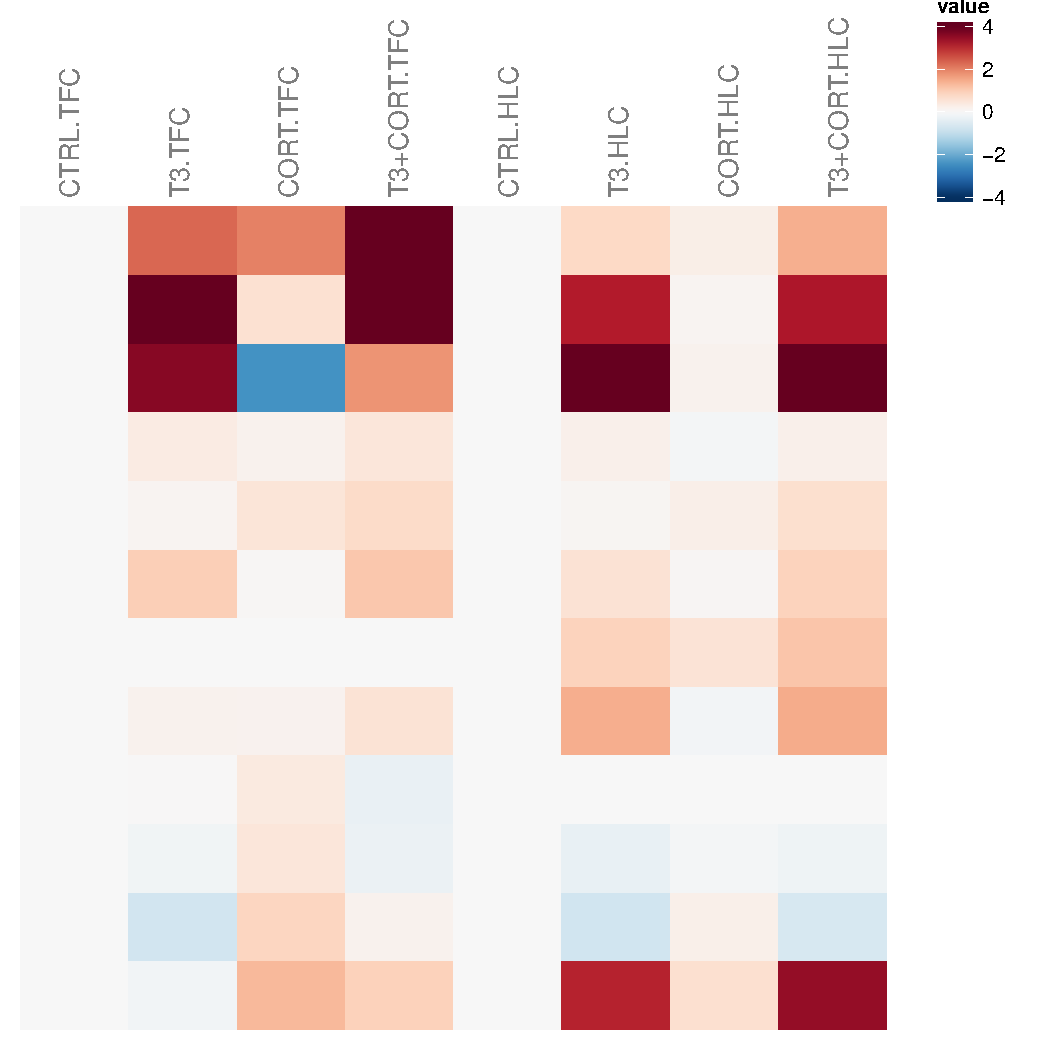
\includegraphics[width=\textwidth]
	{Figures/comparison-tfc-hlc-htsig/comparison-tfc-hlc-htsig-all.pdf}
	\caption{}
	\label{subfig:comparison-tfc-hlc-htsig-all}
\end{subfigure}
~
\begin{subfigure}{0.45\textwidth}
	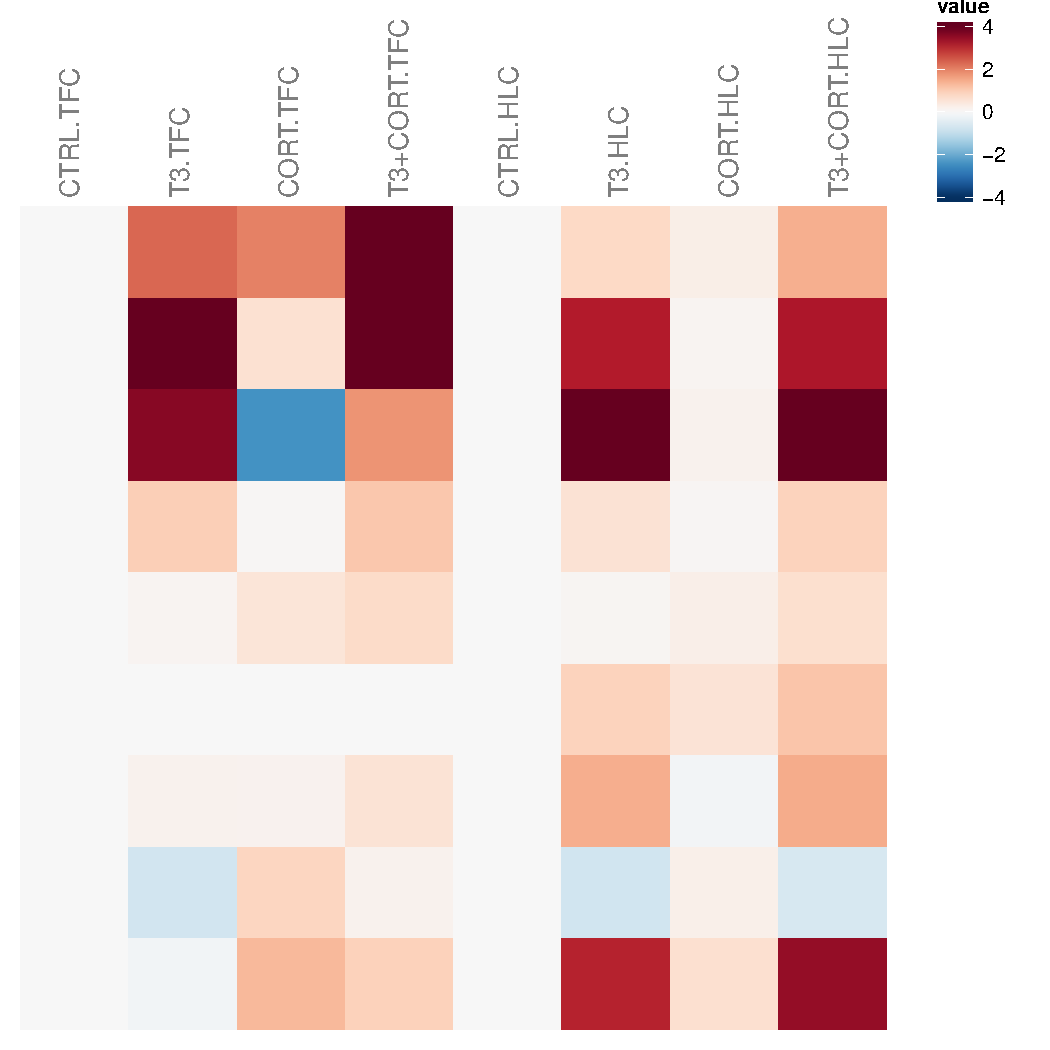
\includegraphics[width=\textwidth]
	{Figures/comparison-tfc-hlc-htsig/comparison-tfc-hlc-htsig-de.pdf}
	\caption{}
	\label{subfig:comparison-tfc-hlc-htsig-de}
\end{subfigure}
\caption[Profils d'expression des gènes impliqués dans la signlisation et le métabolisme des hormones thyroïdiennes]
{
Comparaison des profils d'expression, dans l'épiderme caudal et les bourgeons de membres postérieurs, des gènes impliqués dans la signlisation et le métabolisme des hormones thyroïdiennes.
\ref{subfig:comparison-tfc-hlc-htsig-all} Tous les gènes
\ref{subfig:comparison-tfc-hlc-htsig-de} Sélection des gènes différentiellement exprimés dans au moins une condition.
}
\label{fig:comparison-tfc-hlc-htsig}
% ===========================================================
%
% BOTTOM caption
% ------------------------
\end{figure}
% ------------------------
%
% SIDE caption
% ------------------------
%\end{SCfigure}
% ------------------------

La majorité d'entre eux (9) sont différentiellement exprimés dans au moins un traitement (\autoref{subfig:comparison-tfc-hlc-htsig-de}), dont 4 spécifiquement dans les \glspl{hlb}.
Il est intéressant de noter que l'expression d'un seul gène est fortement réprimée par les \glspl{gc}, et uniquement dans le \gls{tf}.
Il s'agit de \gls{dio3}, qui fait partie des gènes co-régulés par les deux hormones.
Les autres gènes dont l'expression est potentialisée ou antagonisée par les \glspl{ht} et les \glspl{gc} incluent \gls{dio2} et \gls{mct}8 dans le \gls{tf}; \gls{trb}, \gls{rxr}$\beta$ et \gls{rxr}$\gamma$, \gls{dio2} et \gls{dio3} dans les \glspl{hlb}.
A noter que dans la \autoref{fig:comparison-tfc-hlc-htsig}, \gls{dio3} dans les \glspl{hlb} n’apparaît pas comme ``antagonisé'' car les facteurs d'induction ont été écrêtés à $\pm 4$ afin de ne pas affecter le contraste pour les autres gènes.
\par
L'expression de \gls{dio2} est induite par la \gls{t3} et la \gls{cort} dans le \gls{tf} ($log_2(FC)=2,31$ respectivement) et dans une moindre mesure dans les \glspl{hlb}.
En présence des deux hormone, sont expression est potentiée dans les deux tissus.
\par
En ce qui concerne \gls{dio3}, elle est fortement induite par la \gls{t3} dans le \gls{tf} ($log_2(FC)=3,65$) et dans les \glspl{hlb} ($log_2(FC)=5,76$).
Alors que la \gls{cort} a peu d'effet sur sa transcription dans les \glspl{hlb}, elle réprime fortement sa transcription dans le \gls{tf} ($log_2(FC)=-2,39$).
Enfin, dans les deux tissus, le co-traitement induit une induction de la transcription moins forte que par la \gls{t3} seule ($log_2(FC)=1,79$ dans le \gls{tf} ; $log_2(FC)=4,52$ dans les \glspl{hlb}).
\par
les \glspl{ht} induisent fortement la transcription de \gls{lat}1 dans les \glspl{hlb} ($log_2(FC)=3,1$) mais pas dans le \gls{tf}.
Alors que \gls{mct}10 est légèrement induit par la \gls{t3} dans les deux tissus, l'expression de \gls{mct}8 n'est pas affectée par la \gls{t3}.
Le traitement à la \gls{cort} induit marginalement la transcription de \gls{lat}1 et \gls{oatp}1c1 dans les \gls{hlb} et de \gls{mct}8 dans le \gls{tf}, mais augmente de près d'un facteur 2,5 l'expression de \gls{lat}1 dans le \gls{tf}.
Enfin, le co-traitement induit la sur-expression de \gls{mct}8 et 10 dans les \glspl{hlb} et le \gls{tf}.
L'expression de \gls{lat}1 lors du co-traitement suit les niveaux d'induction provoqués par la \gls{t3} seule dans les \glspl{hlb} et par la \gls{cort} seule dans le \gls{tf}.

%[1] "../heatmap_thyroid.hormone_tailfin-hindlimb"
%[1] "../go.thyroid-hormone.tfc   ---   ../go.thyroid-hormone.hlc"
%[1] "pre-filter"
%[1] 11 25
%[1] 11 25
%[1] 12  8
%pdf
%  2
%[1] "post-filter"
%[1]  5 25
%[1]  9 25
%[1] 9 8
\end{section}

\end{chapter}

\end{document}